% -*- root: ../paper.tex -*-

The \systemname knowledge-base is initially populated with a collection of example data sets.
This starting point produces low quality structure, requring careful curation of training data, as well as expert-provided heuristics.
This is intended to be an ongoing process, with continuous feedback from experts and users incrementally refining the knowledge-base.
In this section we outline the design of an interface that streamlines knowledge-base refinement, starting with a collection of random data
The central elements of this interface are 
(1) Visualizing the current quality of the knowledge base;
(2) Identifying problem name/match-quality function pairs;
(3) Refining records in the knowledge base by removing or merging existing data, or adding expert knowledge.

\begin{figure}
	\centering
	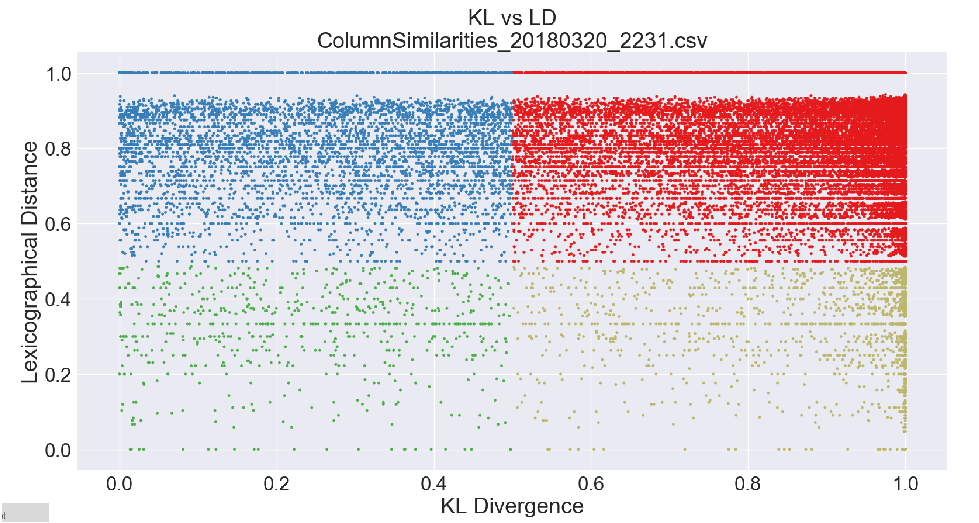
\includegraphics[width=1\columnwidth]{graphics/KBUI}
	\caption{Knowledge base UI/scatter plot}
	\label{fig:Knowledge base user interface}
\end{figure}


\begin{figure}
\begin{tabular}{r|l}
\textbf{How Y modifies X} & $(\namesymbol_x \oplus \namesymbol_y)(T_A)$ \\\hline
X Or Y & $max(\namesymbol_x(T_A), \namesymbol_y(T_A))$\\
X And Y & $\namesymbol_x(T_A) \cdot \namesymbol_y(T_A)$\\
X Unless Y & $min(\namesymbol_x(T_A), \namesymbol_y(T_A))$\\
Y Instead of X & $\namesymbol_y(T_A)$\\
Y Suggests X & $1-(1-\namesymbol_x(T_A))(1-\namesymbol_y(T_A))$
\end{tabular}
\caption{Example augmentation modifiers}
\label{fig:modifiers}
\end{figure}

\tinysection{Modifiers}
Expert knowledge in the knowledge-base is encoded in two parts: 
(1) A quality-match function that provides a heuristic encoding of the expert knowledge, and 
(2) An augmentation modifier that indicates how the new quality match function is to be combined with the existing one.  
Figure~\ref{fig:modifiers} illustrates several example modifiers together with intuitive phrasings of each.  
For example, if the expert heuristic defines an unrelated approach to matching columns, the highest match value is used.


\subsection{Common Refinement Challenges}
We analyzed 179, picked at random from upper left quadrant and the lower right quadrant of figure~\ref{fig:Knowledge base user interface}. The upper left quadrant of the scatter plot consists of data with low KL divergence and high lexicographical distance. The lower right quadrant of the scatter plot consists of data with high KL divergence and low lexicographical distance.Data was tagged(~\ref{fig:Data tags for lower right quadrant}) according to the issues identified. We will discuss these challenges in detail.

\begin{figure}[H]
	\centering
	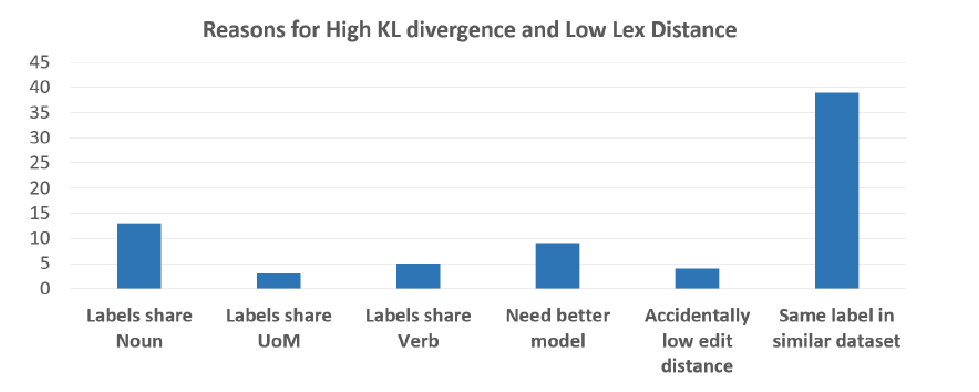
\includegraphics[width=0.8\columnwidth]{graphics/Lower_right_quad}
	\caption{Data tagging for points in lower right quadrant}
	\label{fig:Data tags for lower right quadrant}
\end{figure}

\subsubsection{Challenge 1: Need better model for describing data distribution}
Data distributions were categorized as either uniform or normalized. We analyzed the CDF(figure~\ref{fig:Distribution 1} and figure~\ref{fig:Distribution 2}) of data distribution for each column from the points identified from quadrant one and four of the scatter plot. 
Suggestion: Based on the CDF we identified that a better description of data distribution is required (lognorm, zipfian, etc.).

\begin{figure}[H]
	\centering
	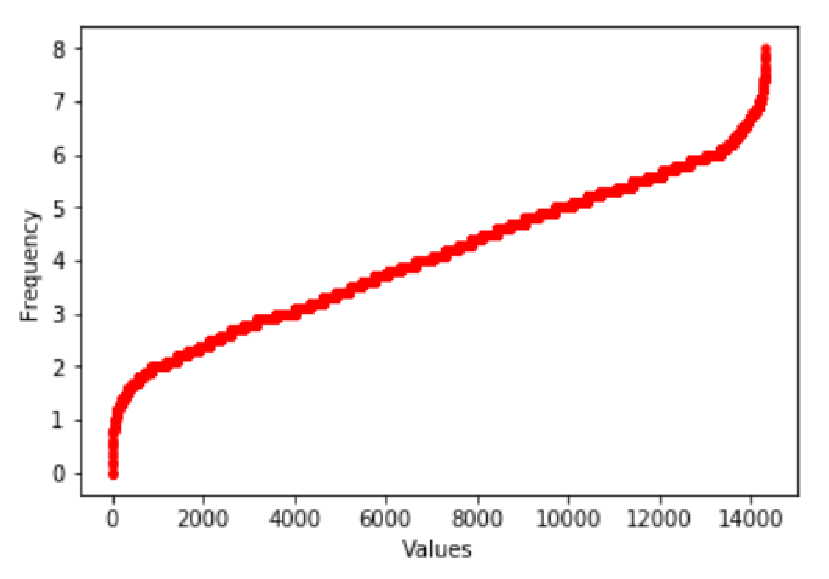
\includegraphics[width=0.8\columnwidth]{graphics/Challenge1_1}
	\caption{CDF of data distribution of column BIGGA\_AVG}
	\label{fig:Distribution 1}
\end{figure}

\begin{figure}[H]
	\centering
	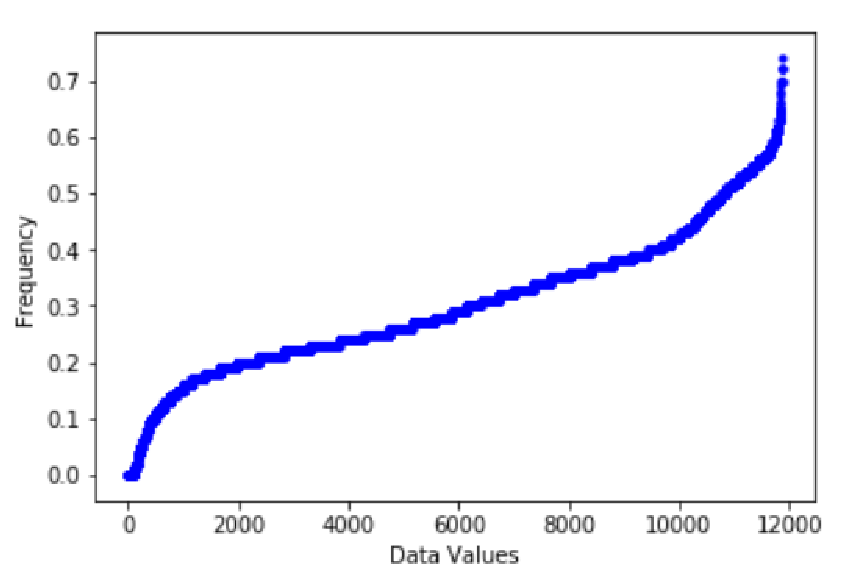
\includegraphics[width=0.8\columnwidth]{graphics/Challenge1_2}
	\caption{CDF of data distribution of column BIGGA\_AVG\_I}
	\label{fig:Distribution 2}
\end{figure}

\subsubsection{Challenge 2: Same column name in similar dataset}
Among the datasets used for this case study, we had two similar datasets in biodiversity domain. Both datasets consisted of data about flora and fauna from two different regions, but same column names. Out of 79 points in the lower right quadrant, 33 were tagged in this category.
Suggestion: A method to differentiate same column names in different datasets is required.

\subsubsection{Challenge 3: Column names share measuring units}
Column names from the agriculture dataset shared measuring units like hectare and tonnes, these points (3 out of 79) resulted in different data distribution (high KL divergence) and low lexicographical distance due to measuring unit being present in the column names. For example: FRUITHECTARES and VEGHECTARES share the measuring units in the column names which causes the lexicographical distance to be low.
Suggestion: Remove the measuring units from column names.

\subsubsection{Challenge 4: Column names share noun}
Some of the column names (13 out of 79) had nouns in common. For instance, BigGameHunting\_RecreationDemand dataset has a column BG\_Demand and MigratoryBirdHunting\_RecreationDemand has a column MB\_Demand. Since the column names share noun, comparing these strings results in low lexicographical distance, but the data distribution are different.
Suggestion: Remove the shared nouns from column names.


\subsubsection{Challenge 5: Column names share verb}
Few column names had words like avg, mean, total, etc. appended at with the names. BAT\_AVG and TAVG share the verb AVG which results in in low lexicographical distance.
Suggestion: Create a list of stop words and remove those from column names.

\subsubsection{Challenge 6: Ngram Overestimation of column names}
Column WTFL\_AVG from biodiversity\_SW\_NHDPv2 and WET\_AG from Wet550\_2017 are classified as similar based on NGram comparison. 
Solution: Use different string comparison function and compare the results.
